%   Filename    : chapter_4.tex 
\chapter{Preliminary Results/System Prototype}
A prototype LoRA implementation was created on Google Colab. 
This uses zephyr-7b-beta model as the base model for finetuning and a part of the ultrachat dataset as the training dataset.
The zephyr-7b-beta model was chosen as it is one of the best performing model after LoRA finetuning \cite{zhao2024loraland310finetuned}.
\begin{figure}
    \caption{Code snippet of the prototype}
    \centering
    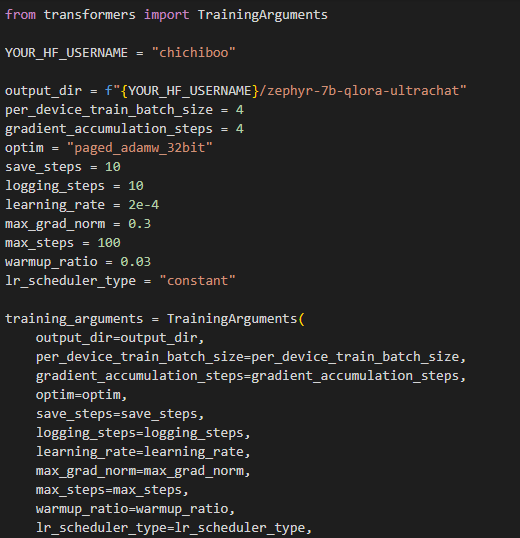
\includegraphics{qlora-snippet}
\end{figure}

This snippet is based on the fine-tuning guides available on HuggingFace and the PEFT guides on several websites.
This prototype only uses 100 iterations to train the model based on the ultrachat dataset.
Most of the parameters used in this prototype is the same with the examples but it establishes a proof of concept on the usage of Google Colab as a potential training platform and the ability of LoRA to improve generative results.

\begin{table}[h!]
	\caption{Difference between Generated Answers of the Base and LoRA Fine-Tuned Model} \vspace{0.25em}
	\centering
	\renewcommand{\arraystretch}{1.2} % Adjusts row spacing
	\begin{tabular}{@{}lp{0.85\linewidth}@{}}
		\hline
		\textbf{Before LoRA:} & \\
		USER: & Can you explain contrastive learning in machine learning in simple terms for someone new to the field of ML? \\
		ASSISTANT: & Contrastive learning is a machine learning technique that involves training a model to learn from data that is similar to the target data. The model is trained to identify patterns in the data that are similar to the target data, and to use those patterns to make predictions about new data. \\
		\hline
		\textbf{After LoRA:} & \\
		USER: & Can you explain contrastive learning in machine learning in simple terms for someone new to the field of ML? \\
		ASSISTANT: & Contrastive learning is a technique in machine learning that uses a technique called contrastive loss to train a model. The idea is to train a model to distinguish between similar and dissimilar data. In contrastive learning, a model is trained to distinguish between a pair of similar data, such as a pair of images, and a pair of dissimilar data, such as a pair of different images. The model is trained to minimize the loss, which is the difference between the similarity and dissimilarity of the data. In contrast, traditional machine learning techniques, such as supervised learning, are trained to distinguish between different types of data, such as a classification or regression task. In summary, contrastive learning is a technique in machine learning that uses a technique called contrastive loss to train a model to distinguish between similar and dissimilar data, which is different from traditional machine learning techniques, such as supervised learning. \\
		\hline
	\end{tabular}
\end{table}
